\documentclass{article}
\usepackage{amsmath,amsfonts,amssymb,tikz,tkz-graph}
\usetikzlibrary{positioning}
\title{MATH 222 Assignment Five}
\author{Oliver Tonnesen\\V00885732}
\date{November 16, 2018}
\begin{document}
\maketitle
\renewcommand{\thesubsection}{\thesection.\alph{subsection}}
\section{} % Section 1
First, we show that for any $m,n\in\mathbb{Z}$ such that $m=n+1$ or $m=n+2$,
$\gcd(m,n)<3$.\\\\
Recall B\'ezout's identity: $\gcd(m,n)$ is the smallest positive integer $d$
such that $d=mp+nq$, $p,q\in\mathbb{Z}$.\\\\
Case 1: $m=n+1$\\
\begin{align*}
	d&=np+(n+1)q\\
	&=np+nq+q\\
	&=(p+q)n+q\\
	&=1&\qquad\text{When $q=1$ and $p=-1$.}
\end{align*}
Since $d$ is defined to be the smallest positive integer satisfying the above
equation and 1 is itself the smallest positive integer, we need not justify
any more.\\\\
Case 2: $m=n+2$, where both $m$ and $n$ are even.\\
In this case $\gcd(m,n)$ is trivially 2, since both are by definition divisible
by 2 and their common divisor cannot be greater than the difference of the two
numbers.\\\\
Case 3: $m=n+2$, where both $m$ and $n$ are odd.\\
In this case, we can denote $m=2l-1$ and $n=2l+1$, for some $l\in\mathbb{Z}$.
We know $2l-1$ and $2l+1$ have 1 as a common divisor. We also know that neither
has 2 as a divisor, since both are odd.\\
Suppose there exists some prime number $p\neq1$ such that $p \mid 2l-1$.
Recall that $p$ cannot be 2. So $2l-1=ap$ for some $a\in\mathbb{Z}$. So
$2l+1=ap+2$. $p$ therefore cannot also divide $2l+1$ unless it is 1 or 2, so in
this case $\gcd(m,n)=2$.\\\\
We've shown that any two integers with a difference less than 3 have a greatest
common divisor of at most 2.\\
Claim: There must exist two numbers in $S$ that differ by less than 3.
Proof: We will try to construct a subset of $S$ of size 673 containing no two
pair of numbers with difference less than 3. Naturally we select every third
number of the set, $1,4,7,10,\ldots$ There are
$\big\lfloor\frac{2018}{3}\big\rfloor=672$ numbers in this sequence. Our subset,
however, must contain 673 elements. So by the pigionhole principle, we cannot
construct such a set, and so the claim holds.

\section{} % Section 2
We calculate the range of possible sums of our subsets by adding the fewest
elements of low value and the most elements of high value. In our case these
are $\{1\}$ and $\{108,\ldots,117\}$ respectively, so our range is $[1,1125]$.
Notice that the extreme values of this range (1 and 1125) are only attainable by
a single set, so we can throw them out. Then our new range is $[2,1124]$. The
value 2 can also only be attained by the subset $\{2\}$, so we can remove this
as well. Our final range is $[3,1124]$. This has reduced our range enough to
apply the pigeonhole principle: There are exactly $2^10-2=1022$ nonempty subsets
of $S$, and there are $1124-3=1021$ possible values, so there must exist two
distinct subsets $A$ and $B$ with $s_A=s_B$.

\section{} % Section 3
\subsection{} % Section 3.a
First we analyze the relation: $x+3y$ is odd when exactly one of $x$ or $y$ is
odd. This knowledge will help us prove some of $\mathcal R$'s properties.\\
Reflexive: No. $(1,1)\not\in\mathcal R$.\\
Symmetric: Yes. $(x,y)\in\mathcal R \implies$ one of $x,y$ is odd, so
$(y,x)\in\mathcal R$, since one of $y,x$ is also odd.\\
Antisymmetric: No. $(1,2)\in\mathcal R$ and $(2,1)\in\mathcal R$, but $1\neq2$.\\
Transitive: No. $(1,2)\in\mathcal R$ and $(2,3)\in\mathcal R$ but
$(1,3)\not\in\mathcal R$.

\subsection{} % Section 3.b
Reflexive: Yes. $X\cap\{1,3,6\}$ is always equal to itself.\\
Symmetric: Yes. The set equality operator is commutative, so if
$X\cap\{1,3,6\}=Y\cap\{1,3,6\}$, then $Y\cap\{1,3,6\}=X\cap\{1,3,6\}$.\\
Transitive: Yes. The set equality operator is transitive, so if
$X\cap\{1,3,6\}=Y\cap\{1,3,6\}$ and $Y\cap\{1,3,6\}=Z\cap\{1,3,6\}$, then
$X\cap\{1,3,6\}=Z\cap\{1,3,6\}$.\\
Antisymmetric: No. $(\emptyset,\{2\})\in\mathcal T$ and $(\{2\},\emptyset)\in\mathcal T$,
but $\emptyset\neq\{2\}$.

\section{} % Section 4
\subsection{} % Section 4.a
Reflexive: $|x-2|=|x-2|$\\
Symmetric: $|x-2|=|y-2| \implies |y-2|=|x-2|$\\
Transitive: $|x-2|=|y-2| \land |y-2|=|z-2| \implies |x-2|=|z-2|$\\
All hold by the definition of $=$ on $\mathbb Z$.
\subsection{} % Section 4.b
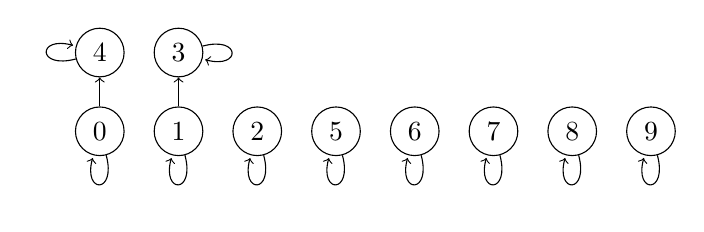
\begin{tikzpicture}[->]
	\node[circle,draw]	(0)	at	(0,0)		{0};
	\node[circle,draw]	(4)	at	(0,1)		{4};
	\node[circle,draw]	(1)	at	(1,0)		{1};
	\node[circle,draw]	(3)	at	(1,1)		{3};
	\node[circle,draw]	(2)	at	(2,0)		{2};
	\node[circle,draw]	(5)	at	(3,0)		{5};
	\node[circle,draw]	(6)	at	(4,0)		{6};
	\node[circle,draw]	(7)	at	(5,0)		{7};
	\node[circle,draw]	(8)	at	(6,0)		{8};
	\node[circle,draw]	(9)	at	(7,0)		{9};
	
	\path	(0)	edge					node[above]	{}	(4);
	\path	(1)	edge					node[above]	{}	(3);
	\path	(0)	edge	[loop below]	node		{}	(1);
	\path	(1)	edge	[loop below]	node		{}	(1);
	\path	(2)	edge	[loop below]	node		{}	(2);
	\path	(3)	edge	[loop right]	node		{}	(3);
	\path	(4)	edge	[loop left]		node		{}	(4);
	\path	(5)	edge	[loop below]	node		{}	(5);
	\path	(6)	edge	[loop below]	node		{}	(6);
	\path	(7)	edge	[loop below]	node		{}	(7);
	\path	(8)	edge	[loop below]	node		{}	(8);
	\path	(9)	edge	[loop below]	node		{}	(9);
\end{tikzpicture}
\subsection{} % Section 4.c
$\{0,4\},\{1,3\},\{2\},\{5\},\{6\},\{7\},\{8\},\{9\}$

\section{} % Section 5
\subsection{} % Section 5.a
There are $|A \times A|=49$ elements that can be in any relation on $A$. Of
these 49, the 7 elements of the form $(x,x)$, $x\in A$ and $(a,b)$ and $(b,c)$
are already chosen, so there are $49-7-1-1$ elements to decide to include or
exclude. So $|\mathcal R|=2^{49-7-1-1}=2^{40}$ such relations are
possible.
\subsection{} % Section 5.b
Each element not of the form $(x,x)$, $x\in A$ included in the relation must be
accompanied by its "pair" (i.e. $(1,2)$ must be with included with $(2,1)$). So
we must make decisions for only one of each pair of non-reflexive elements.
Additionally, $(a,b)$ must be contained, so there are $2^{20-1}=2^{19}$ such
relations.
\subsection{} % Section 5.c
We will count the number of symmetric relations on $A$ and the number of
symmetric and reflexive relations on $A$. We will subtract the latter from the
former to calculate the number of symmetric but not reflexive relations on $A$.\\
Symmetric: $2^{27}$\\
Symmetric and reflexive: $2^{20}$\\
So there are $2^{27}-2^{20}$ such relations.
\subsection{} % Section 5.d
For each pair of non-reflexive elements in A, either or neither, but not both
elements can be in the relation. In other words, there are 3 for each pair
instead of 4. Note that we still have two options for each reflexive element.
Since the relation must contain $(a,b)$, one of the 20 decisions for the pairs
of non-reflexive elements is removed. Since the relation cannot contain $(b,c)$,
another of the 20 decisions for the pairs of non-reflexive elements loses one of
its options. Overall, then, there are $3^{18}\cdot2^7\cdot2$ such relations.
\section{} % Section 6
\subsection{} % Section 6.a
Suppose $\mathcal R_1 \cup \mathcal R_2$ is not symmetric. Then there exists
some $(x,y)\in\mathcal R_1 \cup \mathcal R_2$ such that $(y,x)\not\in\mathcal R_1$
and $(y,x)\not\in\mathcal R_2$. Since $(x,y)\in\mathcal R_1 \cup \mathcal R_2$,
$(x,y)$ must be in one of $\mathcal R_1$ or $\mathcal R_2$, and therefore $(y,x)$
must be in one of $\mathcal R_1$ or $\mathcal R_2$, and therefore must be in
$\mathcal R_1 \cup \mathcal R_2$. This is a contradiction, and so
$\mathcal R_1 \cup \mathcal R_2$ is symmetric.
\subsection{} % Section 6.b
Suppose $(x,y)\in\mathcal R_1 \cap \mathcal R_2$ and $(x,y)\in\mathcal R_1 \cap \mathcal R_2$,
but $x\neq y$. Then $(x,y)\in\mathcal R_1$ and $(y,x)\in\mathcal R_1$. This is a contradiction,
since $x\neq y$ and $\mathcal R_1$ is defined to be antisymmetric, so
$\mathcal R_1 \cap \mathcal R_2$ is antisymmetric.
\subsection{} % Section 6.c
Suppose WLOG that there exists some $x\in A$ such that $(x,x)\not\in\mathcal R_1$.
Then $(x,x)\not\in\mathcal R_1 \cap \mathcal R_2$. This is a contradiction, since
$\mathcal R_1 \cap \mathcal R_2$ is reflexive.
\subsection{} % Section 6.d
False. $A=\{1,2,3\}$, $\mathcal R_1=\{(1,2),(1,3)\}$, $\mathcal R_2=\{(2,3)\}$.

\section{} % Section 7
\subsection{} % Section 7.a
Reflexive: Let $a=a_1a_2\ldots a_n \in A$. For any $1\le i \le n$, $a_i\le a_i$,
so $\mathcal R$ is reflexive.\\
Antisymmetric: Let $a=a_1a_2\ldots a_n,b=b_1b_2\ldots b_n \in A$. If $a\mathcal R b$
and $a\neq b$, then there exists some $1\le k \le n$ such that $a_k=0$ and $b_k=1$.
Thus, $b\not\mathcal R a$, and so $\mathcal R$ is antisymmetric.\\
Transitive: Let $a,b,c\in A$. Suppose $a\mathcal R b$ and $b\mathcal R c$. Then
for every $1\le k \le n$, $a_k \le b_k$ and $b_k \le c_k$, thus $a_k \le c_k$,
and so $a\mathcal R c$. So $\mathcal R$ is transitive.
\subsection{} % Section 7.b
$\;$\\\\\\\\\\\\\\\\\\\\\\\\\\\\\\\\\\
\section{Bonus} % Section 8
We first note that the chess player cannot play more than $11\cdot12=132$ games
during the 77 day period. Let $c_i$ be the number of games played by the $i^\text{th}$
day. Note that $1 \le c_1 \le \ldots \le c_{77} \le 132$. We now must prove that there
must exist some $1 \le i \le j \le 77$ such that $c_j=c_i+21$. So we extend our
original sequence of numbers $c_1,c_2,\ldots,c_{77}$ with the sequence
$c_1+21,c_2+21,\ldots,c_{77}+21$ to get the new sequence
$c_1,\ldots,c_{77},c_1+21,\ldots,c_{77}+21$. This sequence contains 154 elements.
The value of any element in the sequence is in the range [1,132+21], so there are
153 distinct values that any element in the sequence can have. By the pigeonhole
principle, there must exist $i<j$ such that $c_j=c_i+21$, and therefore there
exists a sequence of days over the course of which the chess player plays exactly
21 games.
\end{document}
